% Options for packages loaded elsewhere
\PassOptionsToPackage{unicode}{hyperref}
\PassOptionsToPackage{hyphens}{url}
%
\documentclass[
  ignorenonframetext,
]{beamer}
\usepackage{pgfpages}
\setbeamertemplate{caption}[numbered]
\setbeamertemplate{caption label separator}{: }
\setbeamercolor{caption name}{fg=normal text.fg}
\beamertemplatenavigationsymbolsempty
% Prevent slide breaks in the middle of a paragraph
\widowpenalties 1 10000
\raggedbottom
\setbeamertemplate{part page}{
  \centering
  \begin{beamercolorbox}[sep=16pt,center]{part title}
    \usebeamerfont{part title}\insertpart\par
  \end{beamercolorbox}
}
\setbeamertemplate{section page}{
  \centering
  \begin{beamercolorbox}[sep=12pt,center]{part title}
    \usebeamerfont{section title}\insertsection\par
  \end{beamercolorbox}
}
\setbeamertemplate{subsection page}{
  \centering
  \begin{beamercolorbox}[sep=8pt,center]{part title}
    \usebeamerfont{subsection title}\insertsubsection\par
  \end{beamercolorbox}
}
\AtBeginPart{
  \frame{\partpage}
}
\AtBeginSection{
  \ifbibliography
  \else
    \frame{\sectionpage}
  \fi
}
\AtBeginSubsection{
  \frame{\subsectionpage}
}
\usepackage{lmodern}
\usepackage{amssymb,amsmath}
\usepackage{ifxetex,ifluatex}
\ifnum 0\ifxetex 1\fi\ifluatex 1\fi=0 % if pdftex
  \usepackage[T1]{fontenc}
  \usepackage[utf8]{inputenc}
  \usepackage{textcomp} % provide euro and other symbols
\else % if luatex or xetex
  \usepackage{unicode-math}
  \defaultfontfeatures{Scale=MatchLowercase}
  \defaultfontfeatures[\rmfamily]{Ligatures=TeX,Scale=1}
\fi
\usetheme[]{Hannover}
\usecolortheme{dove}
\usefonttheme{structurebold}
% Use upquote if available, for straight quotes in verbatim environments
\IfFileExists{upquote.sty}{\usepackage{upquote}}{}
\IfFileExists{microtype.sty}{% use microtype if available
  \usepackage[]{microtype}
  \UseMicrotypeSet[protrusion]{basicmath} % disable protrusion for tt fonts
}{}
\makeatletter
\@ifundefined{KOMAClassName}{% if non-KOMA class
  \IfFileExists{parskip.sty}{%
    \usepackage{parskip}
  }{% else
    \setlength{\parindent}{0pt}
    \setlength{\parskip}{6pt plus 2pt minus 1pt}}
}{% if KOMA class
  \KOMAoptions{parskip=half}}
\makeatother
\usepackage{xcolor}
\IfFileExists{xurl.sty}{\usepackage{xurl}}{} % add URL line breaks if available
\IfFileExists{bookmark.sty}{\usepackage{bookmark}}{\usepackage{hyperref}}
\hypersetup{
  pdftitle={Session 1: Multiple linear regression review},
  pdfauthor={Levi Waldron},
  hidelinks,
  pdfcreator={LaTeX via pandoc}}
\urlstyle{same} % disable monospaced font for URLs
\newif\ifbibliography
\usepackage{longtable,booktabs}
\usepackage{caption}
% Make caption package work with longtable
\makeatletter
\def\fnum@table{\tablename~\thetable}
\makeatother
\usepackage{graphicx,grffile}
\makeatletter
\def\maxwidth{\ifdim\Gin@nat@width>\linewidth\linewidth\else\Gin@nat@width\fi}
\def\maxheight{\ifdim\Gin@nat@height>\textheight\textheight\else\Gin@nat@height\fi}
\makeatother
% Scale images if necessary, so that they will not overflow the page
% margins by default, and it is still possible to overwrite the defaults
% using explicit options in \includegraphics[width, height, ...]{}
\setkeys{Gin}{width=\maxwidth,height=\maxheight,keepaspectratio}
% Set default figure placement to htbp
\makeatletter
\def\fps@figure{htbp}
\makeatother
\setlength{\emergencystretch}{3em} % prevent overfull lines
\providecommand{\tightlist}{%
  \setlength{\itemsep}{0pt}\setlength{\parskip}{0pt}}
\setcounter{secnumdepth}{-\maxdimen} % remove section numbering

\title{Session 1: Multiple linear regression review}
\author{Levi Waldron}
\date{}
\institute{CUNY SPH Biostatistics 2}

\begin{document}
\frame{\titlepage}

\hypertarget{learning-objectives-and-outline}{%
\section{Learning objectives and
outline}\label{learning-objectives-and-outline}}

\begin{frame}{Learning objectives}
\protect\hypertarget{learning-objectives}{}

\begin{enumerate}
\tightlist
\item
  identify systematic and random components of a multiple linear
  regression model
\item
  define terminology used in a multiple linear regression model
\item
  define and explain the use of dummy variables
\item
  interpret multiple linear regression coefficients for continuous and
  categorical variables
\item
  use model formulae to multiple linear models
\item
  define and interpret interactions between variables
\item
  interpret ANOVA tables
\end{enumerate}

\end{frame}

\begin{frame}{Outline}
\protect\hypertarget{outline}{}

\begin{enumerate}
\tightlist
\item
  multiple regression terminology and notation
\item
  continuous \& categorical predictors
\item
  interactions
\item
  ANOVA tables
\item
  Model formulae
\end{enumerate}

\end{frame}

\hypertarget{multiple-linear-regression}{%
\section{Multiple Linear Regression}\label{multiple-linear-regression}}

\begin{frame}{Systematic part of model}
\protect\hypertarget{systematic-part-of-model}{}

For more detail: Vittinghoff section 4.2

\[
E[y|x] = \beta_0 + \beta_1 x_1 + \beta_2 x_2 + ... + \beta_p x_p
\]

\begin{itemize}
\tightlist
\item
  \(E[y|x]\) is the expected value of \(y\) given \(x\)
\item
  \(y\) is the outcome, response, or dependent variable
\item
  \(x\) is the vector of predictors / independent variables
\item
  \(x_p\) are the individual predictors or independent variables
\item
  \(\beta_p\) are the regression coefficients
\end{itemize}

\end{frame}

\begin{frame}{Random part of model}
\protect\hypertarget{random-part-of-model}{}

\(y_i = E[y_i|x_i] + \epsilon_i\)

\(y_i = \beta_0 + \beta_1 x_{1i} + \beta_2 x_{2i} + ... + \beta_p x_{pi} + \epsilon_i\)

\begin{itemize}
\tightlist
\item
  \(x_{ji}\) is the value of predictor \(x_j\) for observation \(i\)
\end{itemize}

Assumption: \(\epsilon_i \stackrel{iid}{\sim} N(0, \sigma_\epsilon^2)\)

\begin{itemize}
\tightlist
\item
  Normal distribution
\item
  Mean zero at every value of predictors
\item
  Constant variance at every value of predictors
\item
  Values that are statistically independent
\end{itemize}

\end{frame}

\begin{frame}{Continuous predictors}
\protect\hypertarget{continuous-predictors}{}

\begin{itemize}
\tightlist
\item
  \textbf{Coding:} as-is, or may be scaled to unit variance (which
  results in \emph{adjusted} regression coefficients)
\item
  \textbf{Interpretation for linear regression:} An increase of one unit
  of the predictor results in this much difference in the continuous
  outcome variable

  \begin{itemize}
  \tightlist
  \item
    \emph{additive model}
  \end{itemize}
\end{itemize}

\end{frame}

\begin{frame}{Binary predictors (2 levels)}
\protect\hypertarget{binary-predictors-2-levels}{}

\begin{itemize}
\tightlist
\item
  \textbf{Coding:} indicator or dummy variable (0-1 coding)
\item
  \textbf{Interpretation for linear regression:} the increase or
  decrease in average outcome levels in the group coded ``1'', compared
  to the reference category (``0'')

  \begin{itemize}
  \tightlist
  \item
    \emph{e.g.} \(E(y|x) = \beta_0 + \beta_1 x\)
  \item
    where x=\{ 1 if male, 0 if female \}
  \end{itemize}
\end{itemize}

\end{frame}

\begin{frame}{Multilevel Categorical Predictors (Ordinal or Nominal)}
\protect\hypertarget{multilevel-categorical-predictors-ordinal-or-nominal}{}

\begin{itemize}
\tightlist
\item
  \textbf{Coding:} \(K-1\) dummy variables for \(K\)-level categorical
  variables *
\item
  \textbf{Interpretation for linear regression:} as above, the
  comparisons are done with respect to the reference category
\item
  Testing significance of multilevel categorical predictor: partial
  F-test, a.k.a. nested ANOVA
\end{itemize}

\small

* STATA and R code dummy variables automatically, behind-the-scenes

\end{frame}

\begin{frame}{Inference from multiple linear regression}
\protect\hypertarget{inference-from-multiple-linear-regression}{}

\begin{itemize}
\tightlist
\item
  Coefficients are t-distributed when assumptions are correct
\item
  Variance in the estimates of each coefficient can be calculated
\item
  The t-test of the null hypothesis \(H_0: \beta_1 = 0\) and from
  confidence intervals tests whether \(x_1\) predicts \(y\),
  \emph{holding other predictors constant}

  \begin{itemize}
  \tightlist
  \item
    often used in causal inference to control for confounding: see
    section 4.4
  \end{itemize}
\end{itemize}

\end{frame}

\hypertarget{interaction-effect-modification}{%
\section{Interaction (effect
modification)}\label{interaction-effect-modification}}

\begin{frame}{How is interaction / effect modification modeled?}
\protect\hypertarget{how-is-interaction-effect-modification-modeled}{}

Interaction is modeled as the product of two covariates: \[
E[y|x] = \beta_0 + \beta_1 x_1 + \beta_2 x_2 + \beta_{12} x_1*x_2
\]

\end{frame}

\begin{frame}{What is interaction / effect modification?}
\protect\hypertarget{what-is-interaction-effect-modification}{}

\begin{figure}
\centering
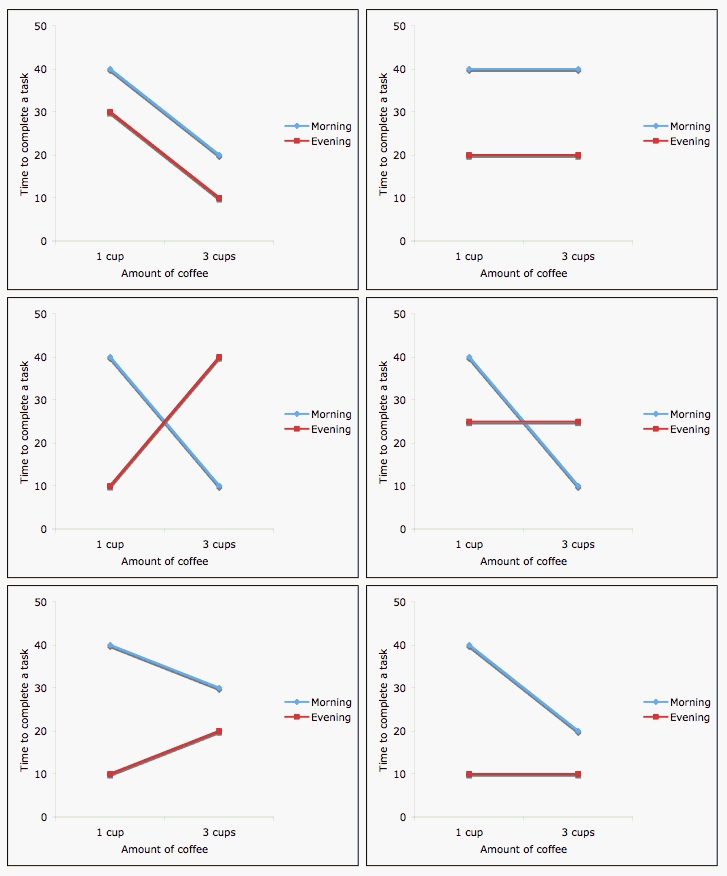
\includegraphics{coffee_interaction.jpg}
\caption{Interaction between coffee and time of day on performance}
\end{figure}

Image credit: \url{http://personal.stevens.edu/~ysakamot/}

\end{frame}

\hypertarget{analysis-of-variance}{%
\section{Analysis of Variance}\label{analysis-of-variance}}

\begin{frame}{Review of the ANOVA table}
\protect\hypertarget{review-of-the-anova-table}{}

\begin{longtable}[]{@{}lllll@{}}
\toprule
Source of Variation & Sum Sq & Deg Fr & Mean Sq & F\tabularnewline
\midrule
\endhead
Model & MSS & k & MSS/k & (MSS/k)/MSE\tabularnewline
Residual & RSS & n-(k-1) & RSS/(n-k-1) &\tabularnewline
Total & TSS & n-1 & &\tabularnewline
\bottomrule
\end{longtable}

\begin{itemize}
\tightlist
\item
  \(k\) = Model degrees of freedom = coefficients - 1
\item
  \(n\) = Number of observations
\item
  \textbf{F} is F-distributed with \(k\) numerator and \(n-(k-1)\)
  denominator degrees of freedom
\end{itemize}

\end{frame}

\hypertarget{model-formulae}{%
\section{Model formulae}\label{model-formulae}}

\begin{frame}[fragile]{What are model formulae?}
\protect\hypertarget{what-are-model-formulae}{}

\href{http://ww2.coastal.edu/kingw/statistics/R-tutorials/formulae.html}{Model
formulae tutorial}

\begin{itemize}
\tightlist
\item
  Model formulae are shortcuts to defining linear models in R
\item
  Regression functions in R such as \texttt{aov()}, \texttt{lm()},
  \texttt{glm()}, and \texttt{coxph()} all accept the ``model formula''
  interface.
\item
  The formula determines the model that will be built (and tested) by
  the R procedure. The basic format is:
\end{itemize}

\begin{quote}
response variable \textasciitilde{} explanatory variables
\end{quote}

\begin{itemize}
\tightlist
\item
  The tilde means ``is modeled by'' or ``is modeled as a function of.''
\end{itemize}

\end{frame}

\begin{frame}{Model formula for simple linear regression}
\protect\hypertarget{model-formula-for-simple-linear-regression}{}

\begin{quote}
y \textasciitilde{} x
\end{quote}

\begin{itemize}
\tightlist
\item
  where ``x'' is the explanatory (independent) variable
\item
  ``y'' is the response (dependent) variable.
\end{itemize}

\end{frame}

\begin{frame}{Model formula for multiple linear regression}
\protect\hypertarget{model-formula-for-multiple-linear-regression}{}

Additional explanatory variables would be added as follows:

\begin{quote}
y \textasciitilde{} x + z
\end{quote}

Note that ``+'' does not have its usual meaning, which would be achieved
by:

\begin{quote}
y \textasciitilde{} I(x + z)
\end{quote}

\end{frame}

\begin{frame}[fragile]{Types of standard linear models}
\protect\hypertarget{types-of-standard-linear-models}{}

\begin{verbatim}
lm( y ~ u + v)
\end{verbatim}

\texttt{u} and \texttt{v} factors: \textbf{ANOVA}\\
\texttt{u} and \texttt{v} numeric: \textbf{multiple regression}\\
one factor, one numeric: \textbf{ANCOVA}

\end{frame}

\begin{frame}{Model formulae cheatsheet}
\protect\hypertarget{model-formulae-cheatsheet}{}

\begin{longtable}[]{@{}lll@{}}
\toprule
symbol & example & meaning\tabularnewline
\midrule
\endhead
+ & + x & include this variable\tabularnewline
- & - x & delete this variable\tabularnewline
: & x : z & include the interaction\tabularnewline
* & x * z & include these variables and their
interactions\tabularnewline
/ & x / z & nesting: include z nested within x\tabularnewline
\textbar{} & x \textbar{} z & conditioning: include x given
z\tabularnewline
\^{} & (u + v + w)\^{}3 & include these variables and\tabularnewline
~ & ~ & all interactions up to three way\tabularnewline
1 & -1 & intercept: delete the intercept\tabularnewline
\bottomrule
\end{longtable}

\end{frame}

\begin{frame}{Model formulae comprehension Q\&A \#1}
\protect\hypertarget{model-formulae-comprehension-qa-1}{}

How to interpret the following model formulae?

y \textasciitilde{} u + v + w + u:v + u:w + v:w\\
y \textasciitilde{} u * v * w - u:v:w\\
y \textasciitilde{} (u + v + w)\^{}2

\end{frame}

\begin{frame}{Model formulae comprehension Q\&A \#2}
\protect\hypertarget{model-formulae-comprehension-qa-2}{}

How to interpret the following model formulae?

\begin{quote}
y \textasciitilde{} u + v + w + u:v + u:w + v:w + u:v:w\\
y \textasciitilde{} u * v * w\\
y \textasciitilde{} (u + v + w)\^{}3
\end{quote}

\end{frame}

\end{document}
